\chapter{Introduction}

\section{Statement of Purpose}

Recognizing activities in videos has become a hot topic over the last years due to the continuous increase of video cameras devices and online repositories. This large amount of data requires an automatic indexing to be accessed after capture. The recent advances in video coding, storage and computational resources have boosted research in the field towards new and more efficient solutions for organizing and retrieving video content.

At the same time, deep learning techniques have been evolving over the last years, bringing new techniques to work with images, and offering solutions to detect and classify objects and activities on them. Somehow, this have made up possible to use this techniques and adding new ones to apply them on videos. Image classification techniques has been broadcasted to obtain the same result on videos, but what videos offer is the challenge to detect temporal actions and activities on it.

The porpuse of this work is face the challenge that videos might offer using deep learning techniques. Rather than focus on activity classification on videos, the aim of this project is to offer a good framework to detect and localize activities on videos. To achieve this goal, the dataset used to fullfill this task will be the ActivityNet Dataset, which offers untrimmed videos which a huge variaty of activities on it.

In particular, this project's main contributions are:
\begin{itemize}
    \item A framework to classify and localize activities on videos using deep learning techniques, more precisely using recurrent neural networks.
    \item Develop techniques to process sequence output from Recurrent Neural Networks, to get the activities' localization on videos.
    \item Explore different configurations of Neural Networks to achieve the best results in activity classification and detection.
    \item Contribute to the research community porting a model to extract features from video from one deep learning framework to another and open sourcing the code.
\end{itemize}

This project has no baseline and all the code and development of deep learning techniques applied to video has been done from scratch.

\section{Requirements and Specifications}

This project has been develop with idea to setup a baseline on this field for future students or researchers to keep working on it. The requirements of this project are the following:
\begin{itemize}
    \item Obtain a Neural Network to classify and temporally localize activities on videos using the ActivityNet Dataset.
    \item Explore different Neural Networks configurations and compare results.
\end{itemize}

Because this project has been developed withou a baseline, no prior specifications were required. Anyway, for the development of this project it has been decided to work with \textit{Python} for development and \textit{Keras} over \textit{Theano}\cite{theano2016theano} as the deep learning framework to use.

\section{Methods and Procedures}



\section{Work Plan}

This project has been planed to follow the packages detailed on this section with the exception of some minor deviations explained on Section~\ref{section:work_plan_deviations}.

\subsection{Work Packages}

\begin{itemize}
    \item WP 1: Project Documentation
    \item WP 2: Research for the State of the Art
    \item WP 3: Dataset to work with
    \item WP 4: Software to use
    \item WP 5: Experimentation and Results Evaluation
    \item WP 6: ActivityNet Challenge 2016 Participation
    \item WP 7: Delivery and Exposition of this project
\end{itemize}

\subsection{Gantt Diagram}

The Gantt diagram of this project's work plan can be found on the Figure~\ref{fig:gantt_diagram}.

\begin{figure}[H]
\begin{center}
% Em falta fer-lo 
%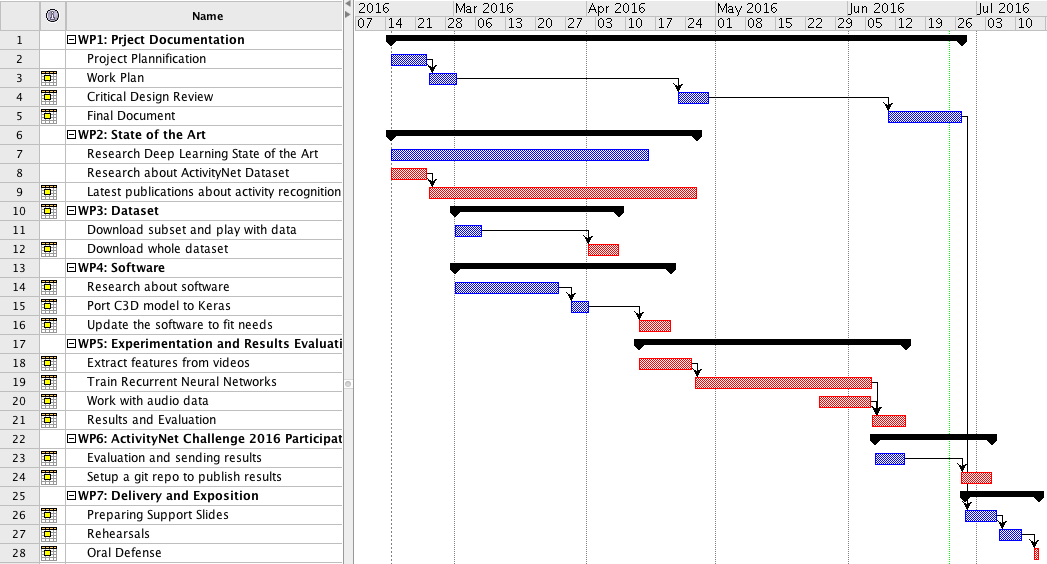
\includegraphics[width=1\linewidth]{img/introduction/gantt_diagram}
\end{center}
\caption{Gantt diagram of this thesis.}
\label{fig:gantt_diagram}
\end{figure}

\section{Work Plan Deviations and Incidents}
\label{section:work_plan_deviations}

The initial plan was thought to use the C3D\cite{tran2014learning} network to work with the video dataset which is based on \textit{Caffe}. But in order to use Recurrent Neural Networks, \textit{Keras} was the best framework to use it, so was necessary to port the original model from one framework to the other.

Another deviation for the plan, has been that, because the huge amount of computational resources required and not available, fine tune the C3D network has not been possible and it has only be used to extract features from the video. Then, all the effort has gone to achieve the best recurrent model to suceed on this project main goal: classify and localize activities in videos.
